% mainfile: ../../../../master.tex
\subsection{Nucleic acid integrity assessment by electrophoresis}
% The part of the label after the colon must match the file name. Otherwise,
% conditional compilation based on task labels does NOT work.
\label{task:20180316_cj0}
\tags{lab,dna,rna}
\authors{cj}
%\files{}
%\persons{}

\subsubsection{1\% Agarose gel preparation}

\begin{enumerate}
\item Measure with erlenmeyer 50~mL of 1\% agarose gel.\sidenote{The 1\% agarose gel is kept at 60\degree C in the gel room.}
\item Warm up the erlenmeyer for 15s in microwave: agarose will be more fluid and it will avoid bubbles when casting the gel
\item Cast the gel with the comb (for 15 wells)
\item Let the gel set for 20 min
\end{enumerate}

\comment{I casted my gels 3 times because the agarose was way to soft and the gel would break when removing the comb. I suspect a new intern prepared the stock solution of 1\% but diluted it too much ... this delayed my progress by almost 2 hours ... In the end, Elísabet prepared a new stock solution that I was able to use.}

\subsubsection{Sample preparation}

In a \gls{pcr} 8-well rack mix:
\begin{itemize}
\item sample of nucleic acid sample according to volumes shown in table \ref{tab:20180316_prep_samples}
\item blue dye (bromothymol blue) according to volumes shown in table \ref{tab:20180316_prep_samples}
\comment{For each sample, the final quantity of nucleic acids is 20~ng.}
\item Tap gently tubes to mix up everything
\item Centrifuge briefly to bring all the liquid to the bottom
\end{itemize}

\begin{table} 
\caption{Volumes needed for nucleic acid migration on agarose gel so that all samples contain 20~ng of nucleic acid}
\label{tab:20180316_prep_samples}
\centering 
\resizebox{\textwidth}{!}{
\begin{tabular}{l l l l l r r r r}
\toprule
Usr & Label & Label colour & Box pos. & Extr. method & Starting material & Qubit\texttrademark~ (\textmu g/mL) & vol. to transfer & vol. dye \\
\midrule
\texttt{CJ} & DNA MP & GREEN & C4 & MasterPure & Micro-algae culture & 3,11 & 6,43 & 3,57
 \\
\texttt{CJ} & RNA MP & GREEN & C5 & MasterPure & Micro-algae culture & 7,20 & 2,78 & 7,22
 \\
\texttt{CJ} & DNA 1802 & PURPLE & C6 & AllPrep & Micro-algae culture & 2,44 & 8,20 & 1,80
 \\
\texttt{CJ} & RNA AP & PINK & C7 & AllPrep & Micro-algae culture & 8,77 & 2,28 & 7,72
 \\
\texttt{CJ} & DNA AP & BLUE & E1 & AllPrep & Micro-algae culture & 5,86 & 3,41 & 6,59
 \\
\texttt{CJ} & RNA AP & BLUE & E2 & AllPrep & Micro-algae culture & 31,50 & 0,63 & 9,37
 \\
\texttt{CJ} & DNA MP & YELLOW & E3 & MasterPure & Micro-algae culture & 18,20 & 1,10 & 8,90
 \\
\texttt{CJ} & RNA MP & YELLOW & E4 & MasterPure & Micro-algae culture & 32,20 & 0,62 & 9,38
 \\
\texttt{CJ} & DNA & NONE & E5 & AllPrep & Micro-algae culture & 7,71 & 2,59 & 7,41
 \\
\texttt{CJ} & RNA & NONE & E6 & AllPrep & Micro-algae culture & 3,94 & 5,08 & 4,92
 \\
\texttt{CJ} & DNA & NONE & E7 & AllPrep & Micro-algae culture & 3,45 & 5,80 & 4,20
 \\
\texttt{CJ} & RNA & NONE & E8 & AllPrep & Micro-algae culture & 14,00 & 1,43 & 8,57
 \\
\texttt{CJ} & MP DNA & PEACH & F1 & MasterPure & Micro-algae culture & 17,00 & 1,18 & 8,82
 \\
\texttt{CJ} & MP RNA & PEACH & F2 & MasterPure & Micro-algae culture & 7,19 & 2,78 & 7,22
 \\

\bottomrule
\end{tabular}
}
\end{table}

\subsubsection{Electrophoresis}

For this electrophoresis migration, we run:
\begin{itemize}
\item 10~\textmu L of each sample 
\item 5~\textmu L of the 1~kb ladder
\item 5~\textmu L of the 2-log ladder
\end{itemize}
\comment{I leave empty lanes between ladders and samples.}

\begin{enumerate}
\item Place the agarose gel into the gel box (electrophoresis unit) containing TAE buffer
\item Load 5~\textmu L of molecular weight ladder into the first and last lane of the gel
\item Load 9~\textmu L of each sample into the additional wells of the gel
\item Run for 65 min with the \gls{eps} 301 at 80~V, 400~mA
\comment{I change the usual settings for a slightly longer run at a lowest voltage (the usual settings I use for electrophoresis are 50 min at 100~V), so that the separation of nucleic acid fragments will be slowlier but clearer.}
\item Remove gel from the migration tank and place in the staining container (a recycled tip box).
\end{enumerate}


\subsubsection{SYBR\cR Gold Staining}

\begin{enumerate}
\item Ensure SYBR\cR gold is properly thawed.
\item Ensure the pH of TAE buffer is between 7.5 and 8
\item Prepare the staining solution at 1X SYBR\cR Gold in TAE buffer.
\comment{I actually use the staining solution solution I made yesterday and kept in aluminium foild at room tempature.}
\item Transfer 100 mL of staining solution in the staining container.
\item Incubate under agitation for 10 to 40 min.
\comment{Gel with DNA was incubated 20 min but since it was hard to take a good picture, I decided to incubate the gel another 20 min to see the difference and it did not change much. Therefore for the gel with RNA, the incubation lasted 30 min.}
\item Visualize your nucleic acid fragments with \gls{uv} lights.
\end{enumerate}
\comment{The CCD camera by BioRad does not work anymore. In the meanwhile, we use transilluminator and take the picture with my cell phone.}

\subsubsection{Results}

\begin{figure}[H] % position of the figure 
    \centering
    \caption{Pictures of the gels after migration}
    \label{fig:20180316_gel_sybr_gold}
    \begin{subfigure}[b]{0.479\textwidth}
        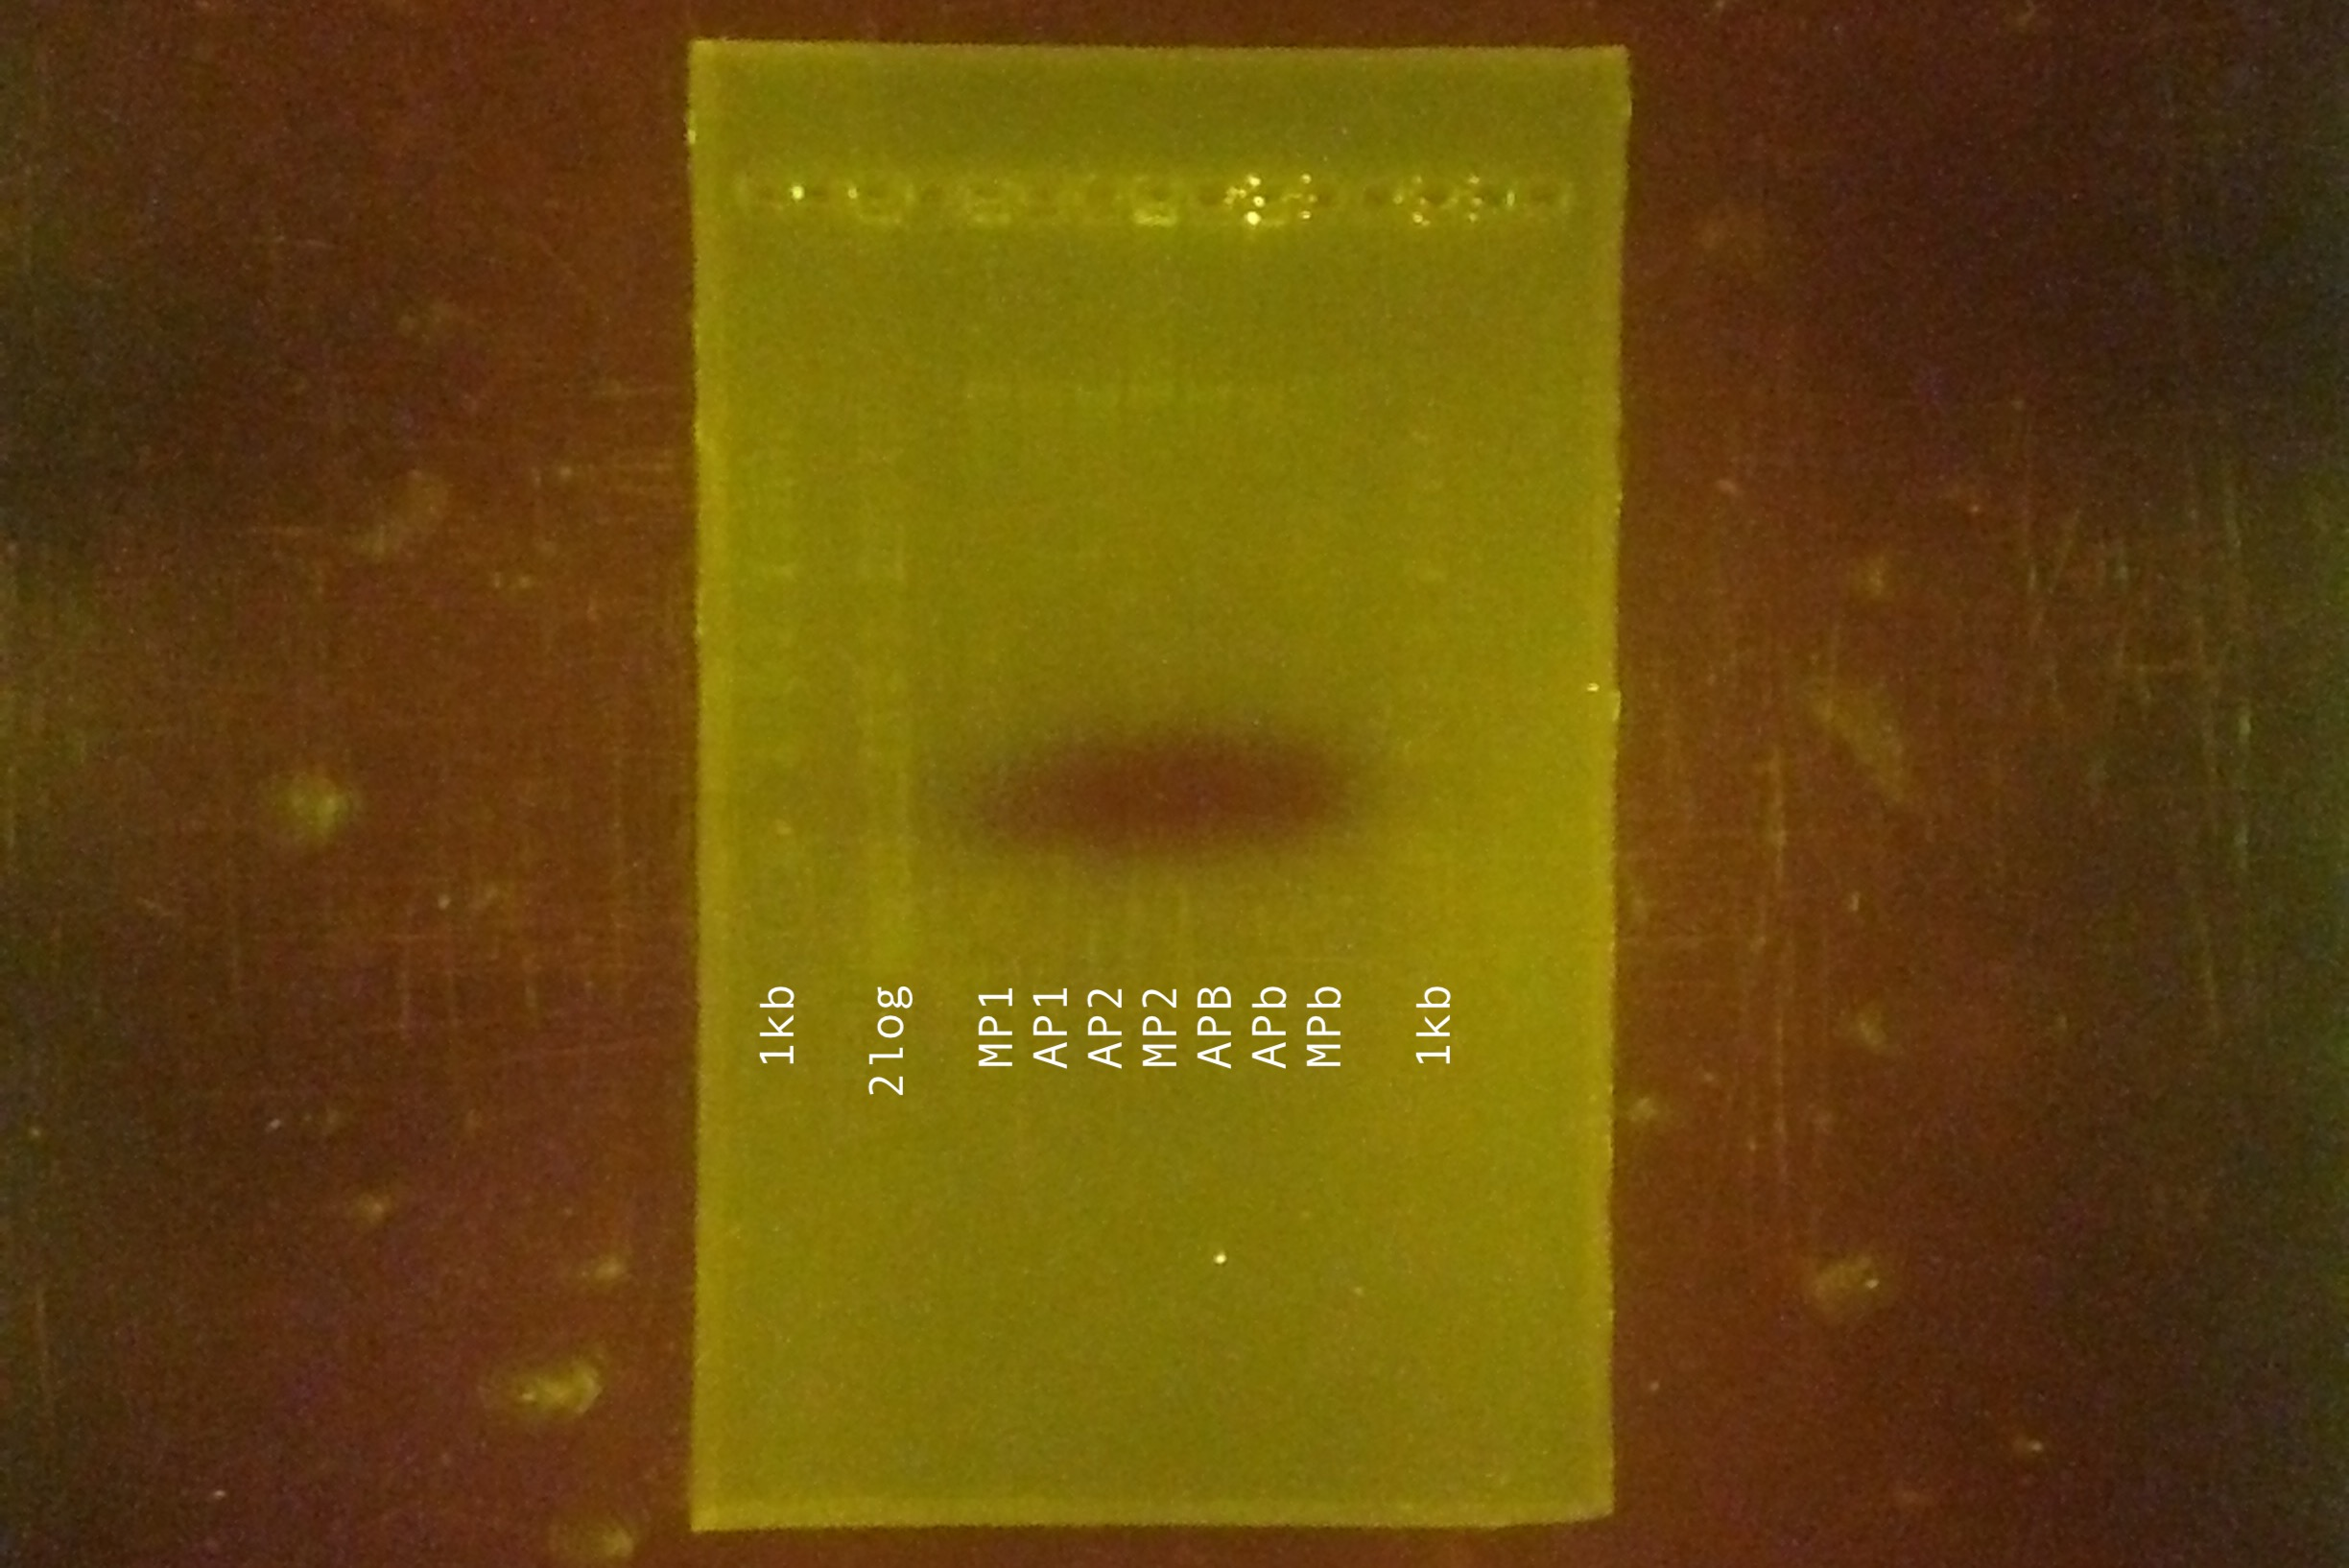
\includegraphics[width=\textwidth]{graphics/pic/20180316_gel_dna_sybr_gold1.JPG}
        \caption{1\% agarose gel with DNA after 20 min. incubation in the 1X SYBR\cR Gold staining solution}
        \label{sfig:20180316_gel_dna_sybr_gold1}
    \end{subfigure}
    ~ 
    \begin{subfigure}[b]{0.24\textwidth}
        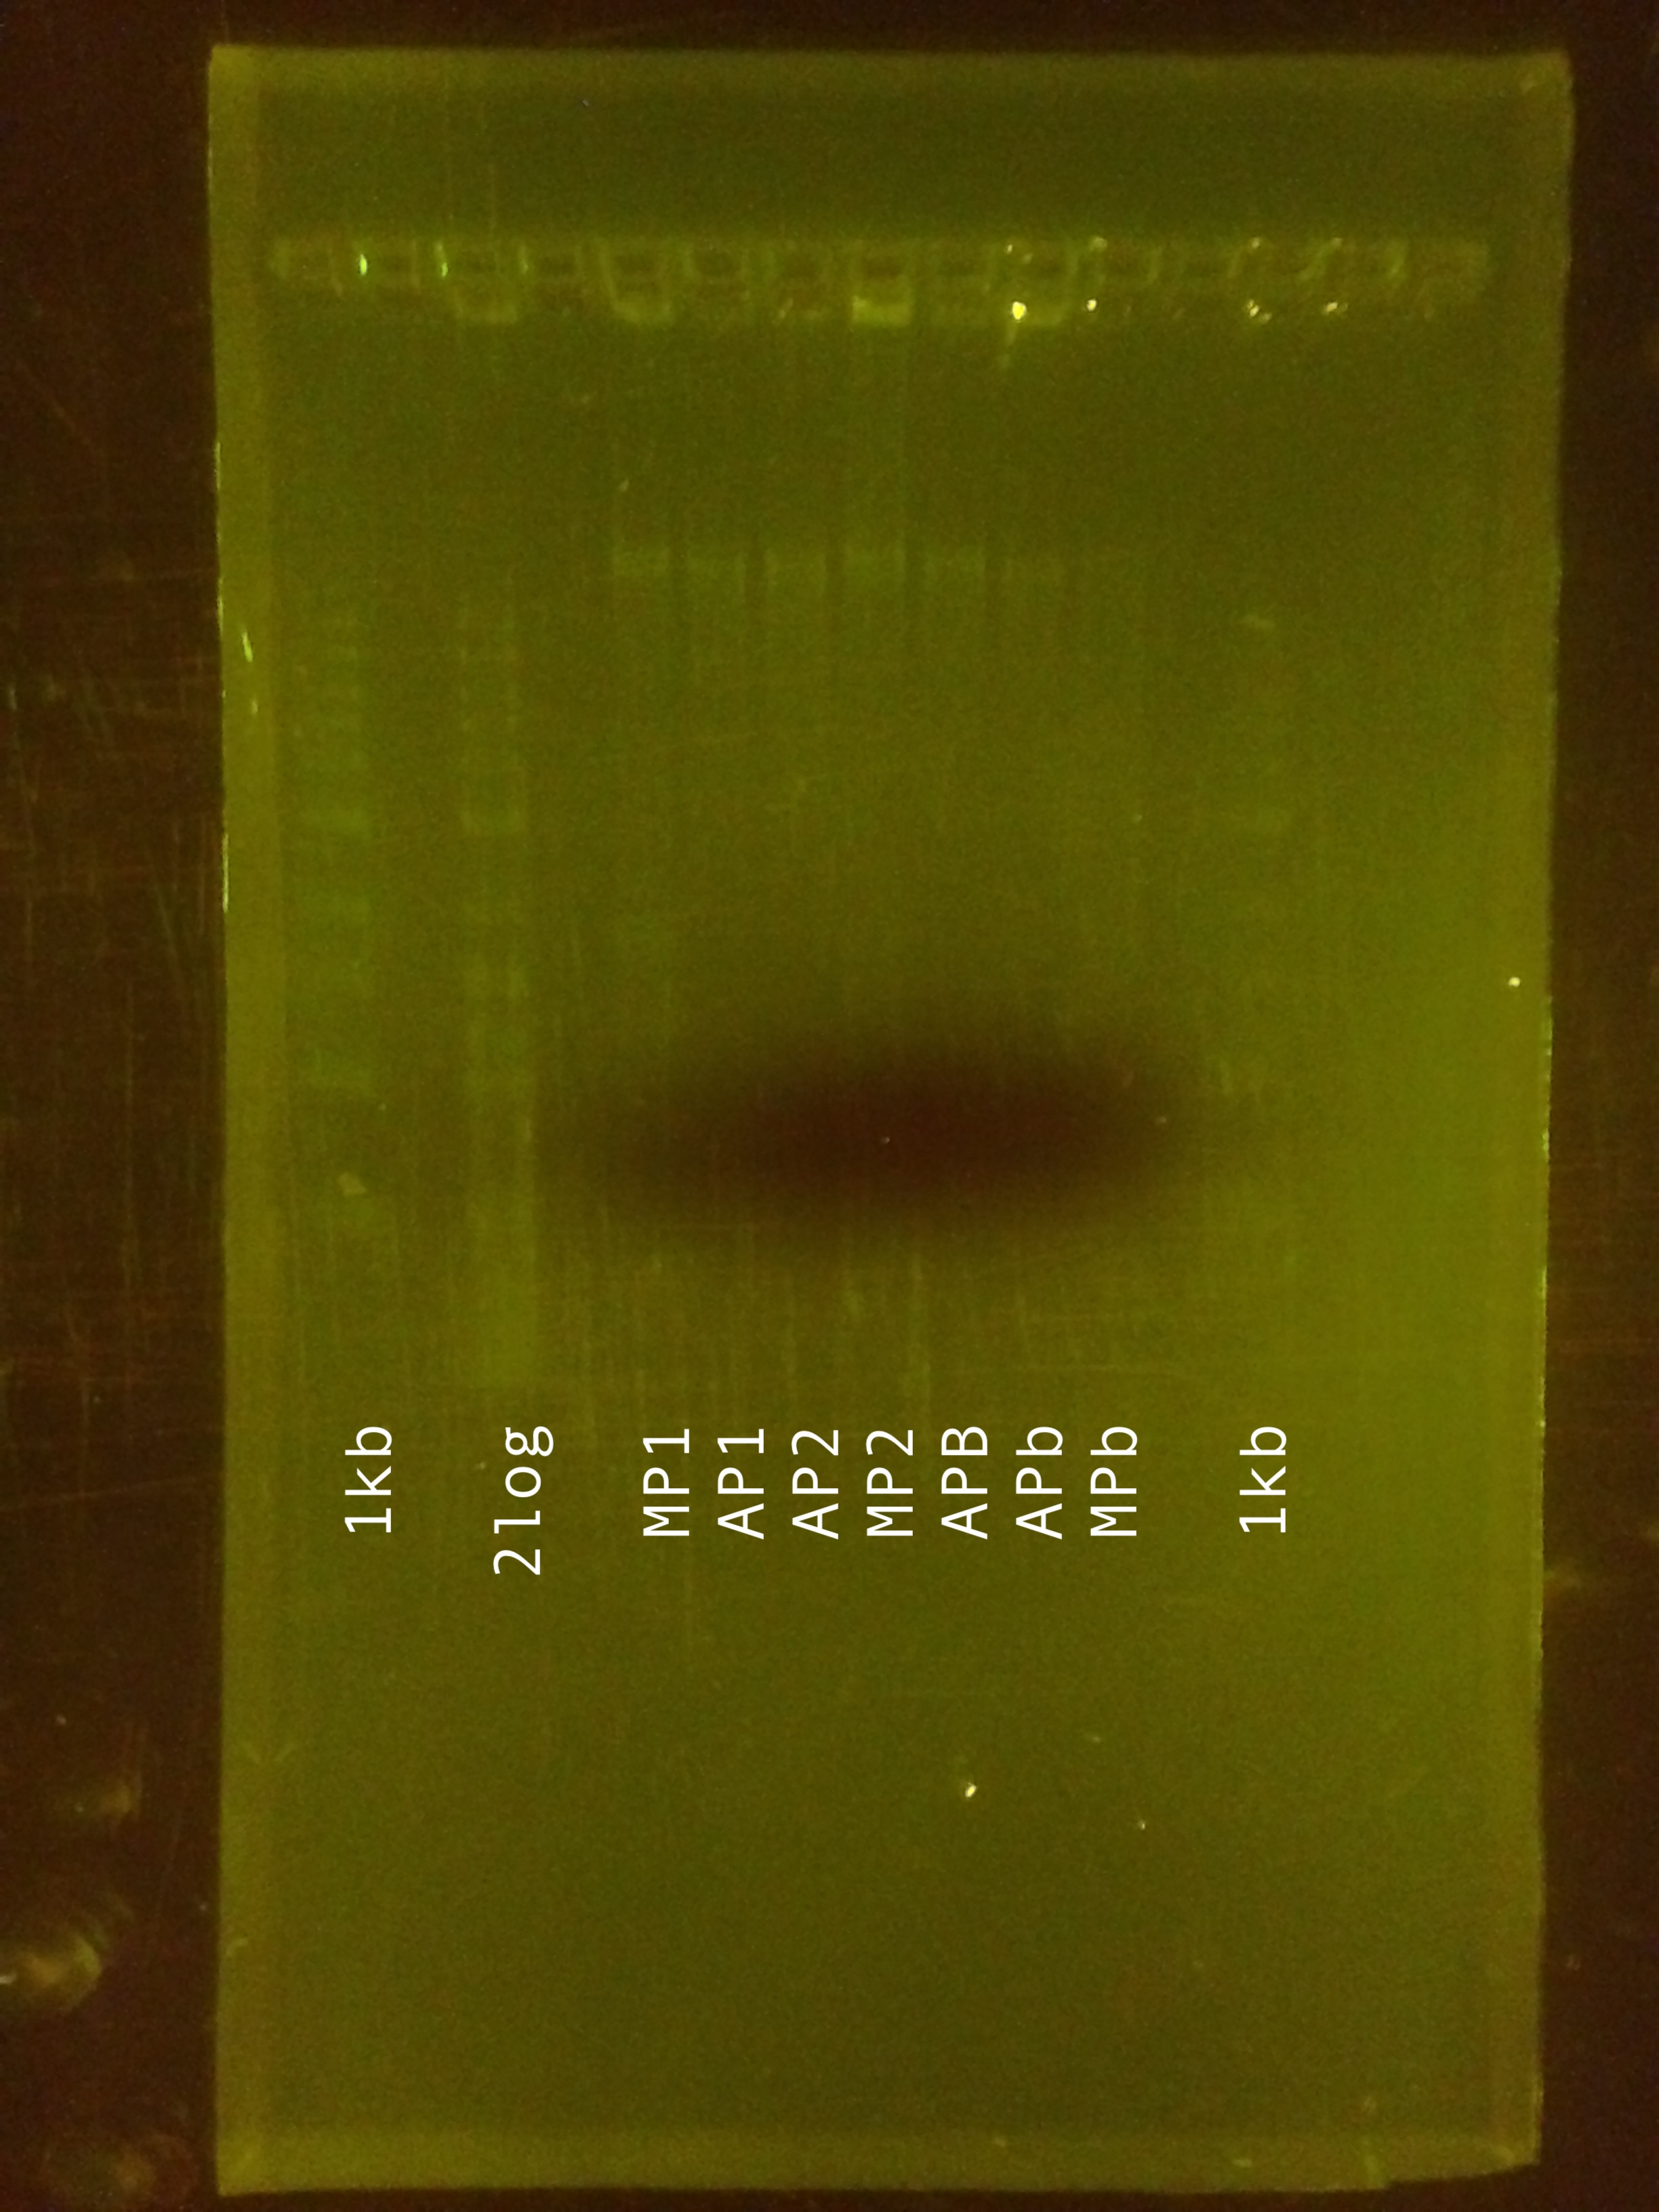
\includegraphics[width=\textwidth]{graphics/pic/20180316_gel_dna_sybr_gold2.JPG}
        \caption{Gel with DNA after 40 min. incubation}
        \label{sfig:20180316_gel_dna_sybr_gold2}
    \end{subfigure}
    ~
     \begin{subfigure}[b]{0.24\textwidth}
        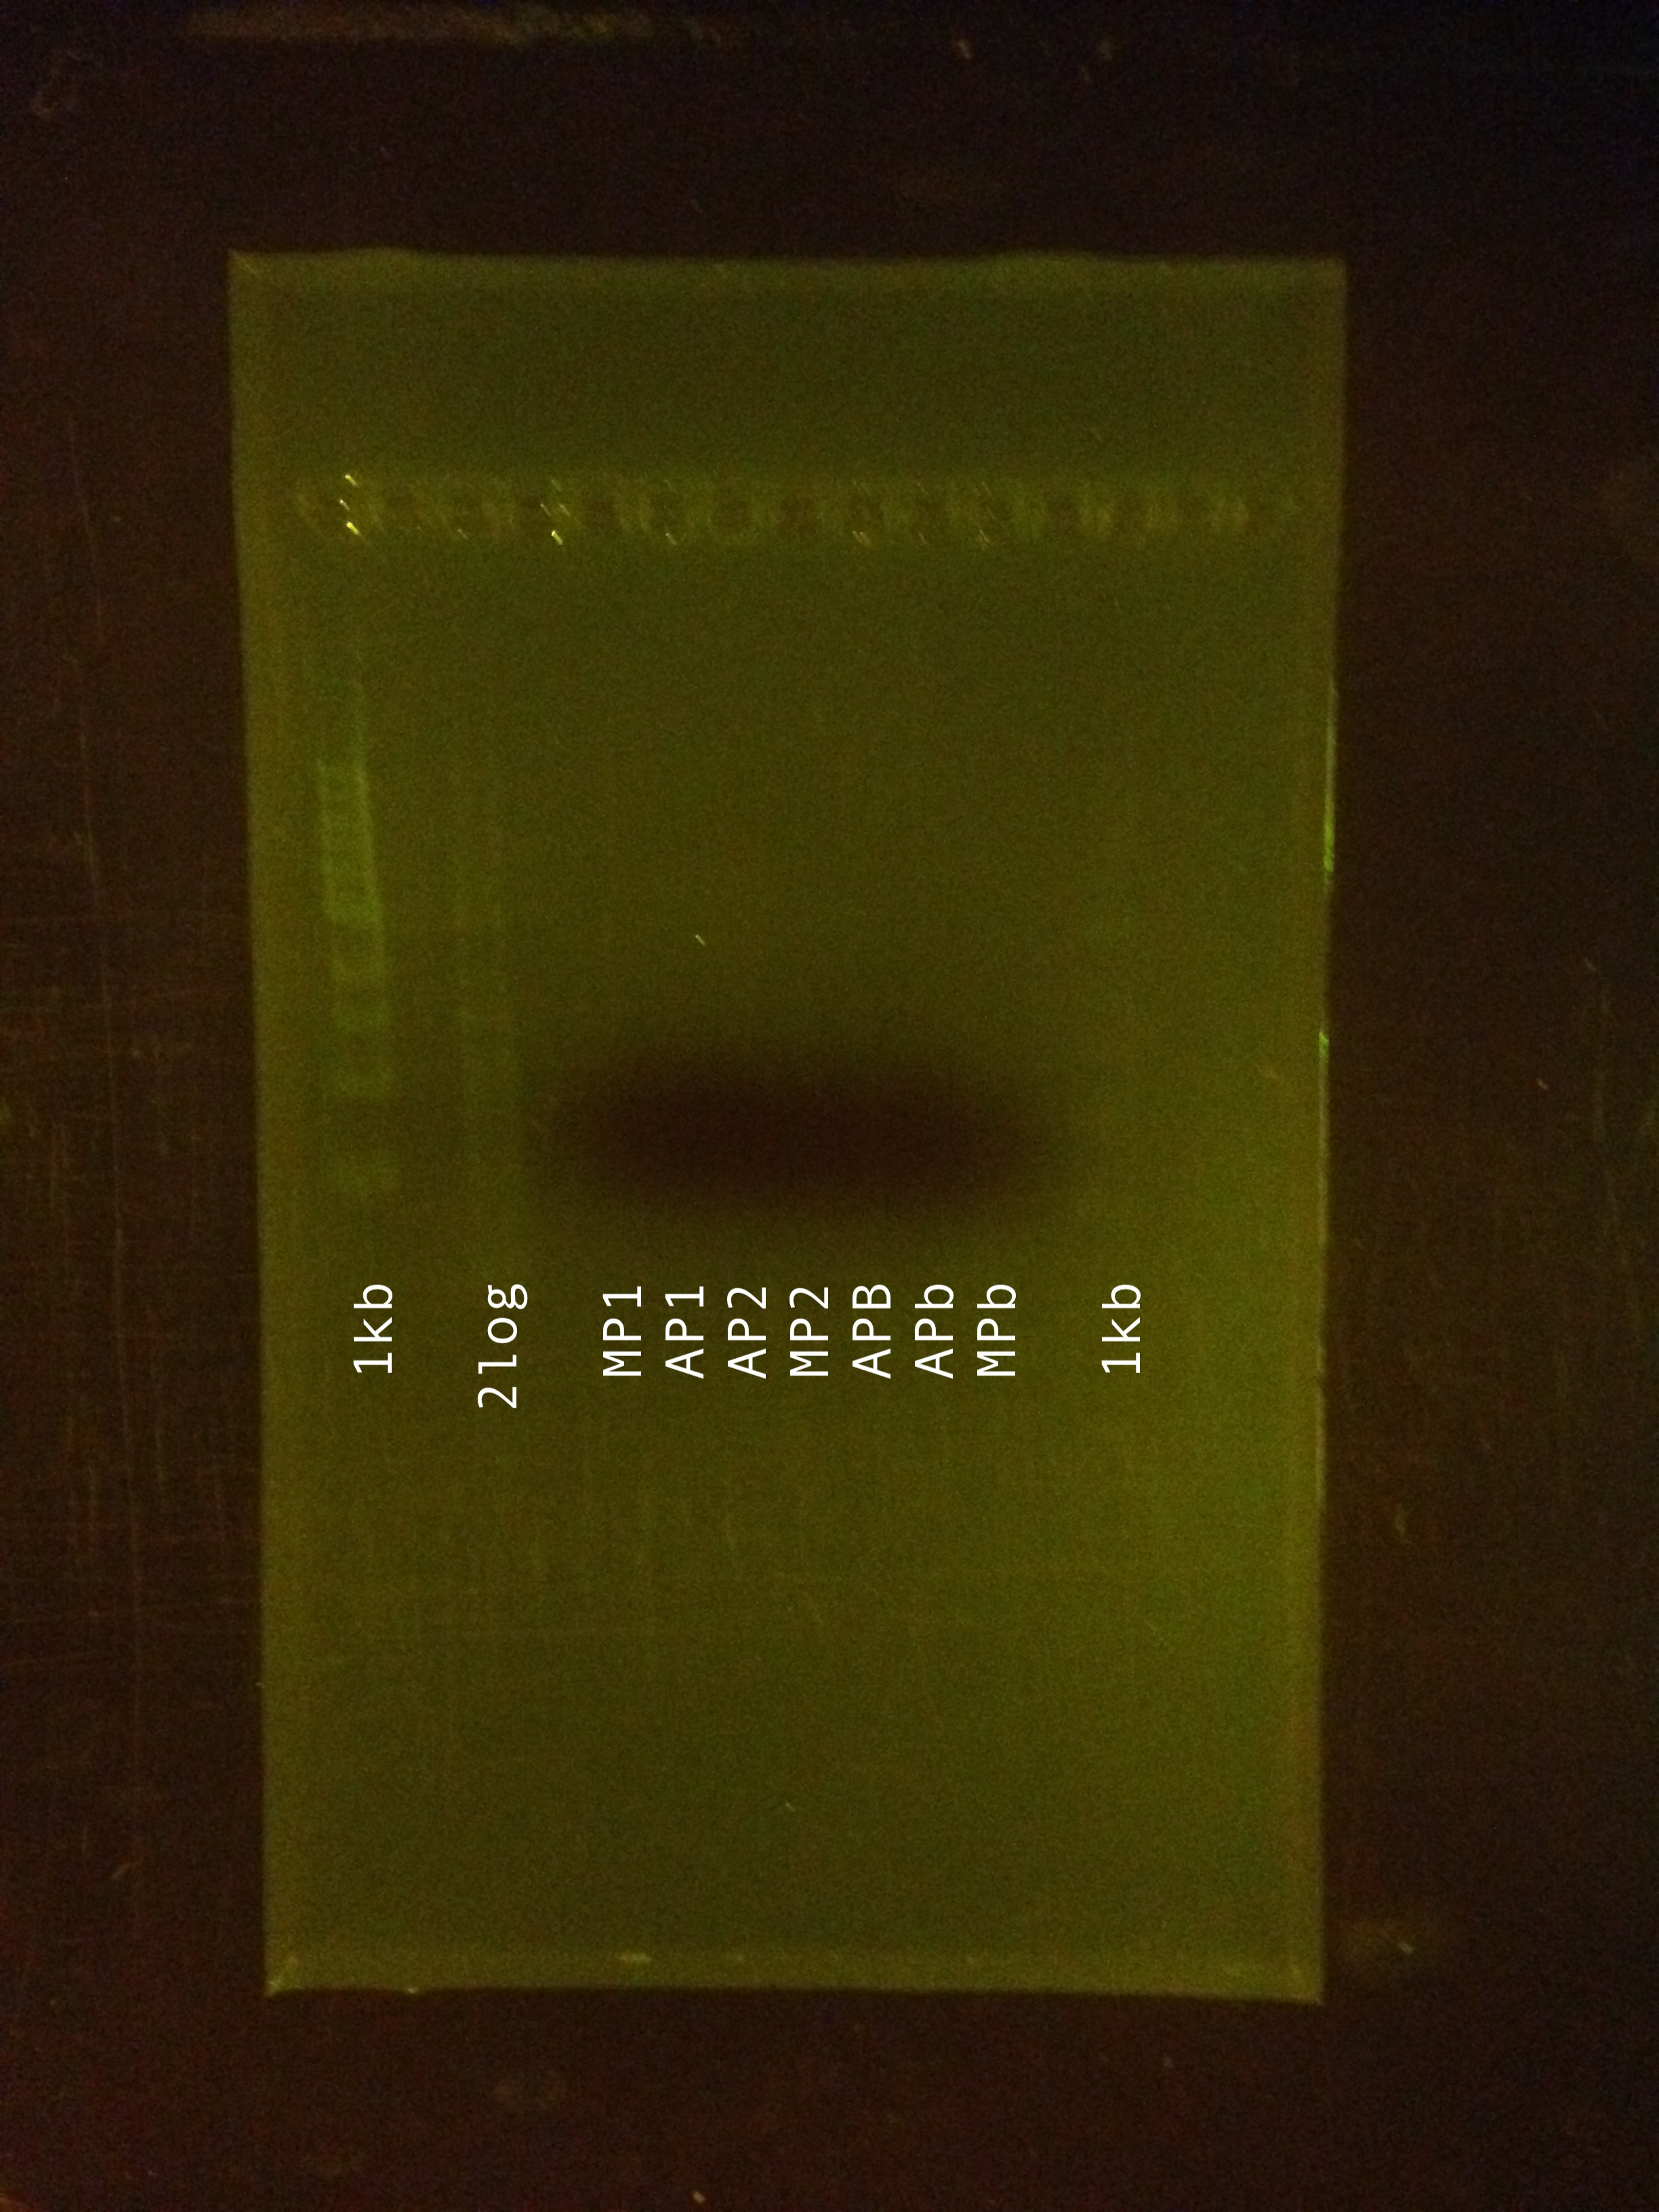
\includegraphics[width=\textwidth]{graphics/pic/20180316_gel_rna_sybr_gold.JPG}
        \caption{Gel with RNA after 30 min. incubation}
        \label{sfig:20180316_gel_rna_sybr_gold}
    \end{subfigure}
\end{figure}

In figures \ref{sfig:20180316_gel_dna_sybr_gold1, sfig:20180316_gel_dna_sybr_gold2}, we can see the ladders and for all samples except the last one (\texttt{MPb}), the bands are rather sharp and clear which indicated a good integrity of DNA. However, for the RNA, there is nothing to see. I suspect that 20 ng is enough to see the genomic DNA since there is one big molecule of genomic DNA while there are multiple type of RNAs. Therefore the 20 ng of RNA end up being splitted into many tiny bands that are therefore too light to be seen. So I must try again with a higher quantity of RNA. 

\subsubsection{Conclusion}

The integrity of the DNA extracted with AllPrep\cR and with MasterPure\texttrademark~ is rather good except for the modified MasterPure\texttrademark~ protocol (involving a gentle bead beating).When working with good quality genomic DNA, 20 ng is enough to visualise the DNA on the gel with SYBR\cR Gold stain. 

Regarding the RNA, I must repeat the experiment with more RNA. I think 100 ng should be good knowing that previously I got really bright results with 300 ng of RNA.

